\chapter{Background Modeling}
\label{chap:modeling}
The study dedicated to the modeling of the major background is shown in this chapter.
The modeling of the MC is needed to be confirmed, thereby data/MC needs to be matched well to estimate the background modeling.
The V+jets is the dominant background for all three channels. 

\section{$m_{jj}^{tag}$ reweighting}
There is a known mis-modelling issue with the Sherpa~2.2.1 V+jets samples. This mis-modelling is seen in the $m^{tag}_{jj}$ distribution as a slope when comparing the data over MC both in merged and the resolved region, as seen in Figure~\ref{fig:2lep_mtag_before_rw}. 
This mis-modeling is founded to be related to the theoretical calculation of the colinear jets. 
The re-weighting is performed to the Z+jets samples for 2-lepton channel, in order to correct this mis-modeling before defining the SRs and CRs. A linear fit to the $m^{tag}_{jj}$ in CRs are performed for each merged and resolved CRs. 

The fit function is defined as:
\begin{equation}
\label{eqn:reweight}
R=p_{0} * m_{jj}^{tag}+p_{1}
\end{equation}
where the R = $data/MC$. The correction is performed only for the Z+jets samples, therefore the other MC samples are subtracted at first. The all samples of mc16a+d+e period is used for reweighting, since there is no much difference in fitted value between mc periods when fitted each period separately. All distributions are first normalized then the correction function (\ref{eqn:reweight}) is derived. Only the difference of the shape is corrected, and difference of the normalization is accounted in the final fit.
The fitted parameter is summarized in the Table~\ref{tab:fit}. These parameters are used as the reweighting factors and applied after the categorizations of the SRs and the CRs. The reweighted distributions are shown in Figure~\ref{fig:2lep_mtag_before_rw}.

\begin{table}[htbp]
 \footnotesize
\begin{center}
\begin{tabular}{ | c | c | c |}
\hline
Parameter & Merged CRVjet & Resolved CRVjet  \\
\hline
$p_{0}$ (slope) [$\GeV^{-1}$] & $(-23.8 \pm 2.5)e^{-5}$ &  $(-17.5 \pm 0.5)e^{-5}$ \\
 \hline
$p_{1}$ (constant)  & $1.298 \pm 0.031$ & $1.187 \pm 0.005$ \\
\hline
\end{tabular}
\caption{\label{tab:fit} Fitted re-weighting parameters for the merged and resolved regions. The errors written here are the uncertainties of the fitted parameters. }
  \end{center}
\end{table}


\begin{figure}[ht]
    \centering
    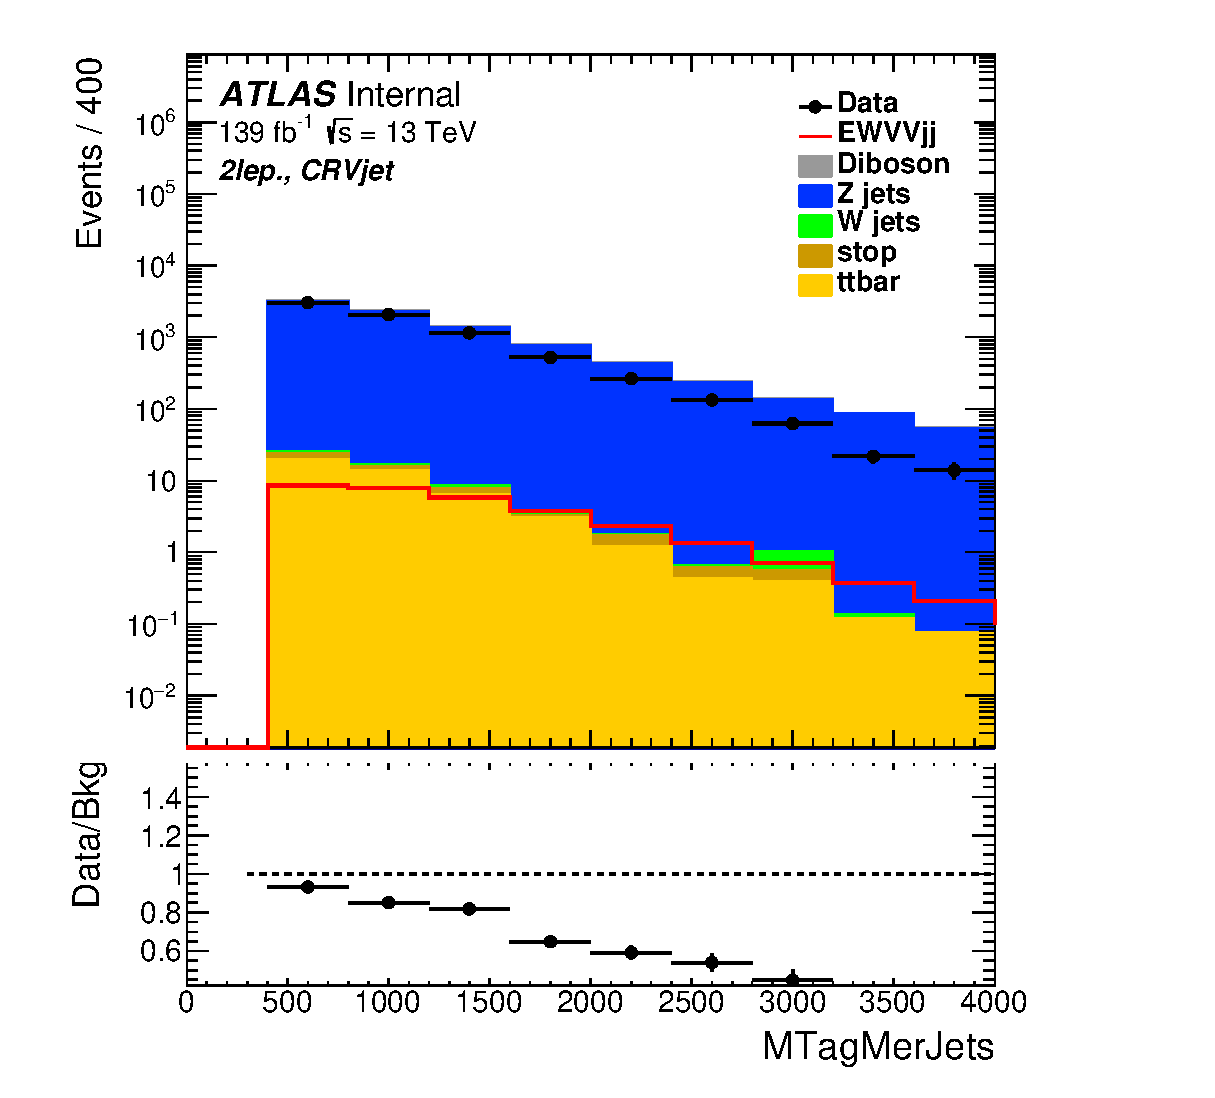
\includegraphics[width=0.45\textwidth]{figures/2lep/reweighting/before_reweighting/C_0ptag1pfat0pjet_0ptv_CRVjet_MTagMerJets_Log.eps}
    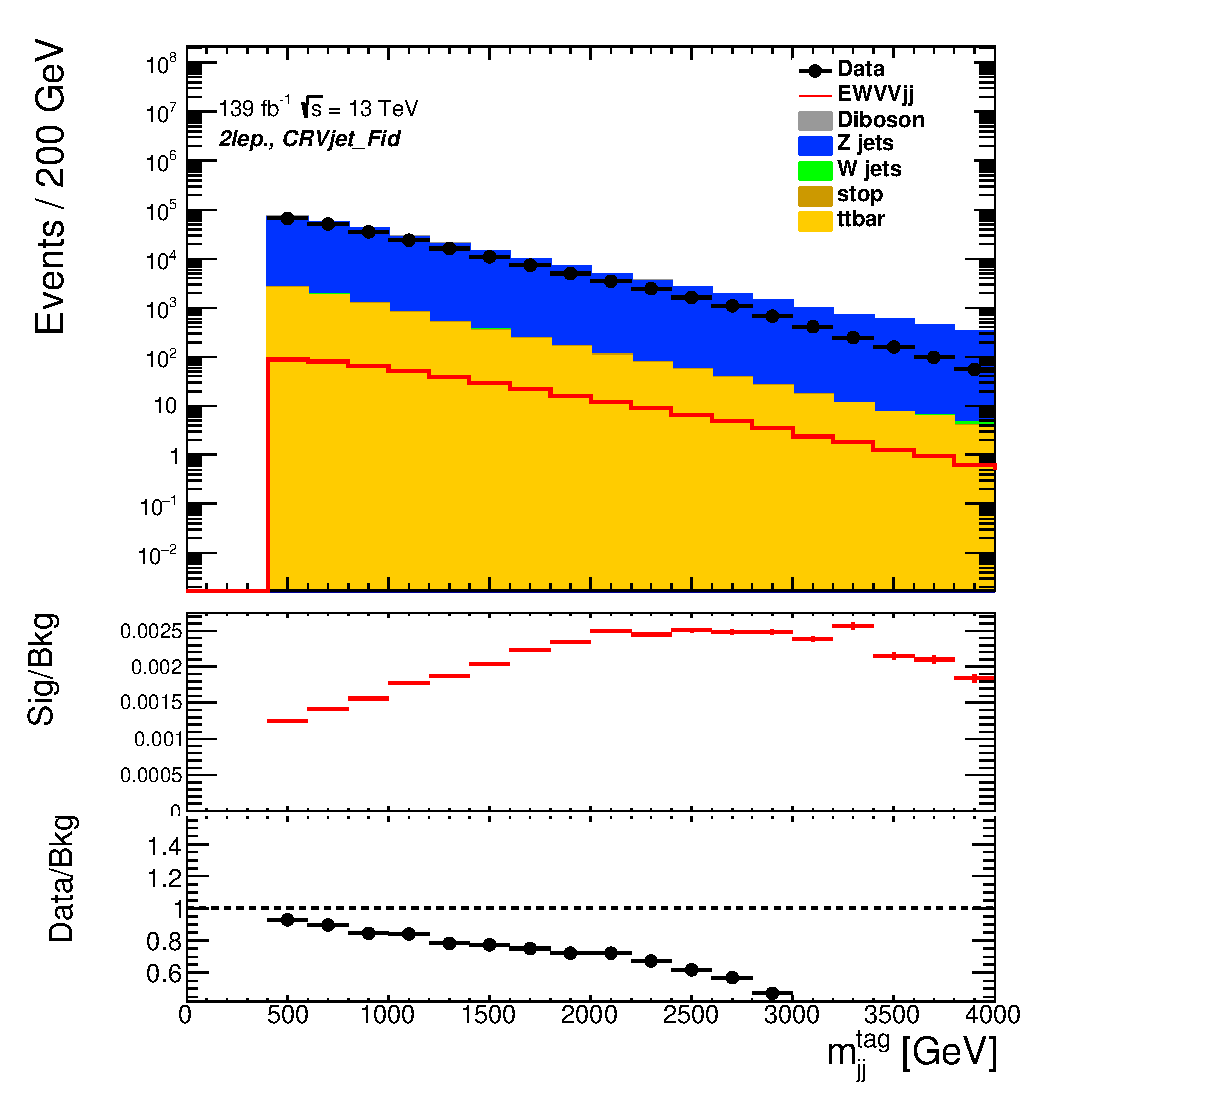
\includegraphics[width=0.45\textwidth]{figures/2lep/reweighting/before_reweighting/C_0ptag2pjet_0ptv_CRVjet_Fid_MTagResJets_Log.eps}
    \caption{ $m^{tag}_{jj}$ distributions before applying reweighting for the merged (a) and resolved (b) control regions in the 2-lepton channel.}
    \label{fig:2lep_mtag_before_rw}
\end{figure}

\begin{figure}[ht]
    \centering
    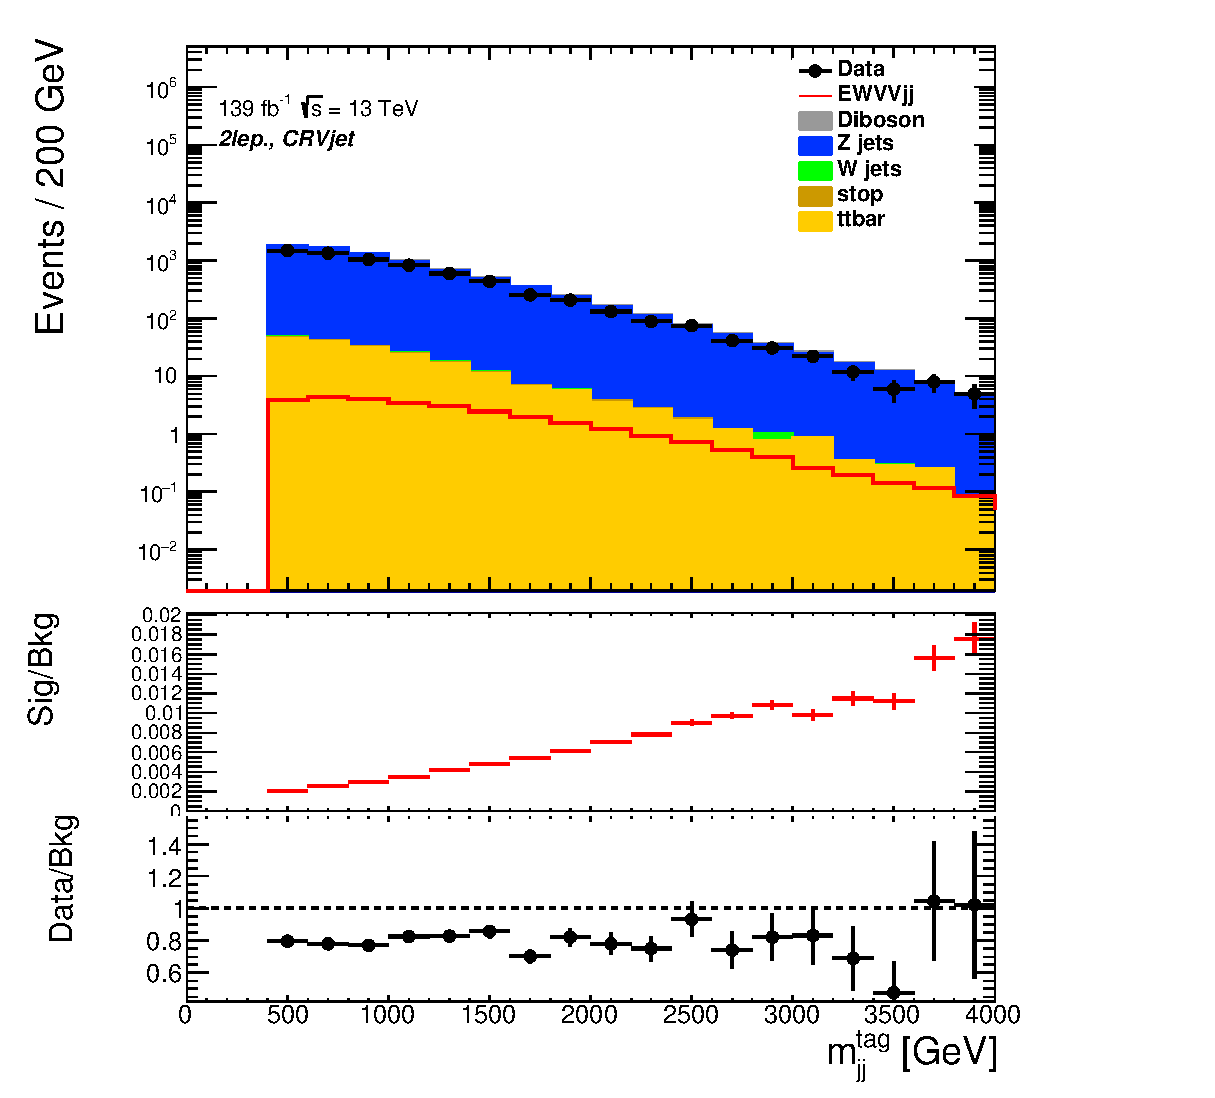
\includegraphics[width=0.45\textwidth]{figures/2lep/reweighting/after_reweighting/C_0ptag1pfat0pjet_0ptv_CRVjet_MTagMerJets_Log.eps}
    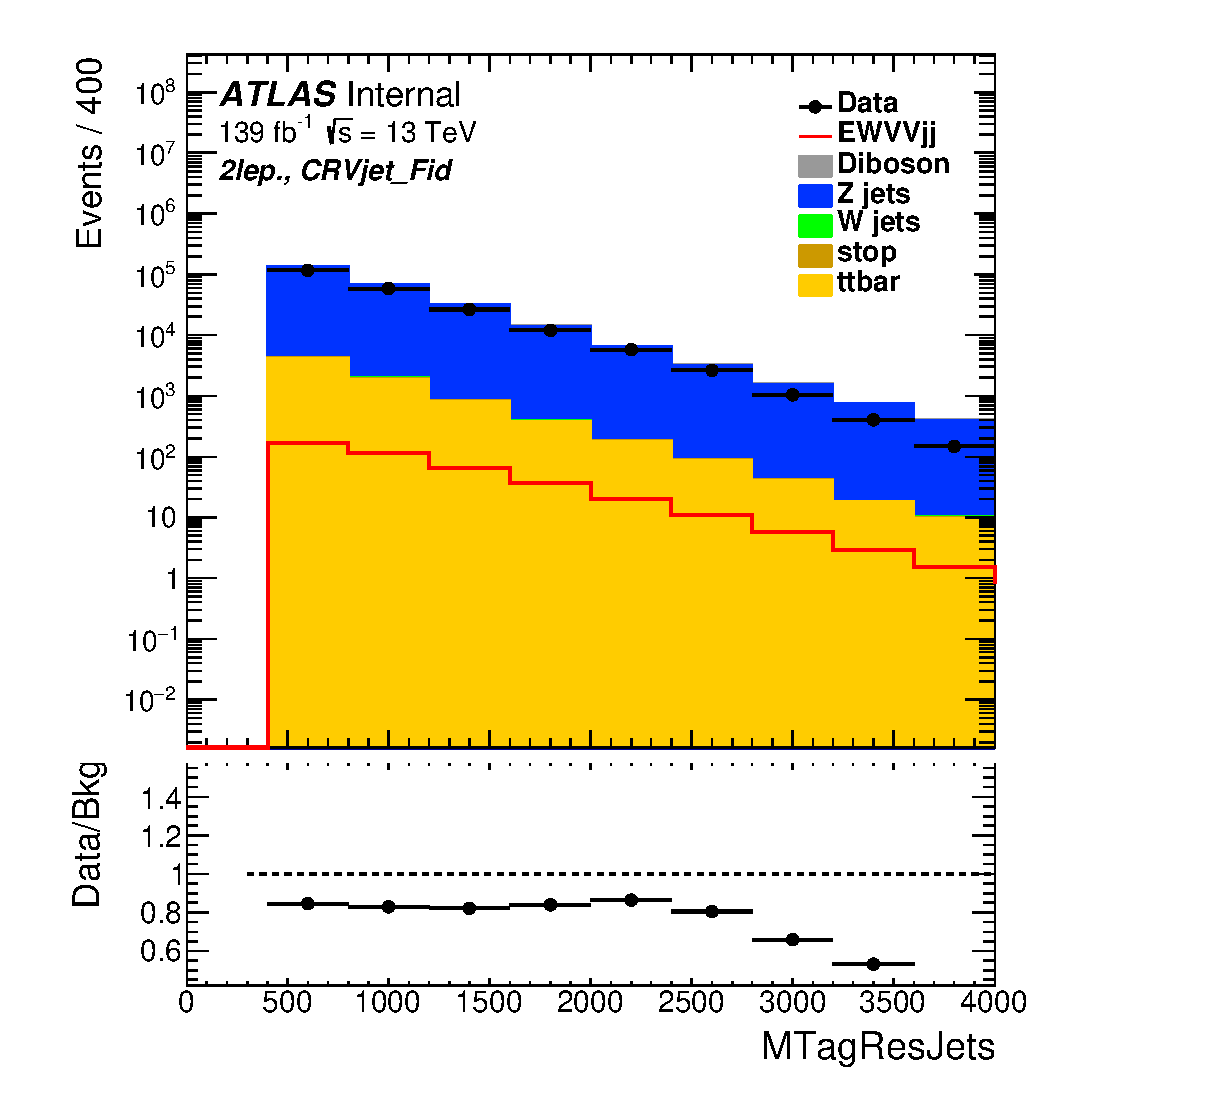
\includegraphics[width=0.45\textwidth]{figures/2lep/reweighting/after_reweighting/C_0ptag2pjet_0ptv_CRVjet_Fid_MTagResJets_Log.eps}
    \caption{ $m^{tag}_{jj}$ distributions after applying reweighting for the merged (a) and resolved (b) control regions in the 2-lepton channel. The slope seen before reweighting is corrected in the Z+jet CR.}
    \label{fig:2lep_mtag_before_rw}
\end{figure}

The uncertainty for this reweighting is assigned in the fitting, considering a 100~\% uncertainty on the linear fit parameters.

%************write something about MadGraph and the dedicated modeling uncertainty here**********
%There is alternative samples using MadGraph instread of Shelpa. The modeling of the MadGraph samples in CRs are shown in Figure.
%The MadGraph has better modeling in our phase space which requires high $m^{tag}_{jj}$. However Shelpa is used as the baseline sample, since it has much statistics.

\section{Z+jets modeling after reweighting}

The $Z$+jets production is the leading background for the 2-lepton channel. The comparison of distributions from data and MC for various kinematic variables after reweighting in the 2-lepton Z+jets merged and resolved control region are shown in Figure \ref{fig:2lep_zjets_merged_CR} and Figure \ref{fig:2lep_zjets_resolved_CR}
respectively. 

% 2-lepton new merged CR - plots
\begin{figure}[ht]
 \centering
   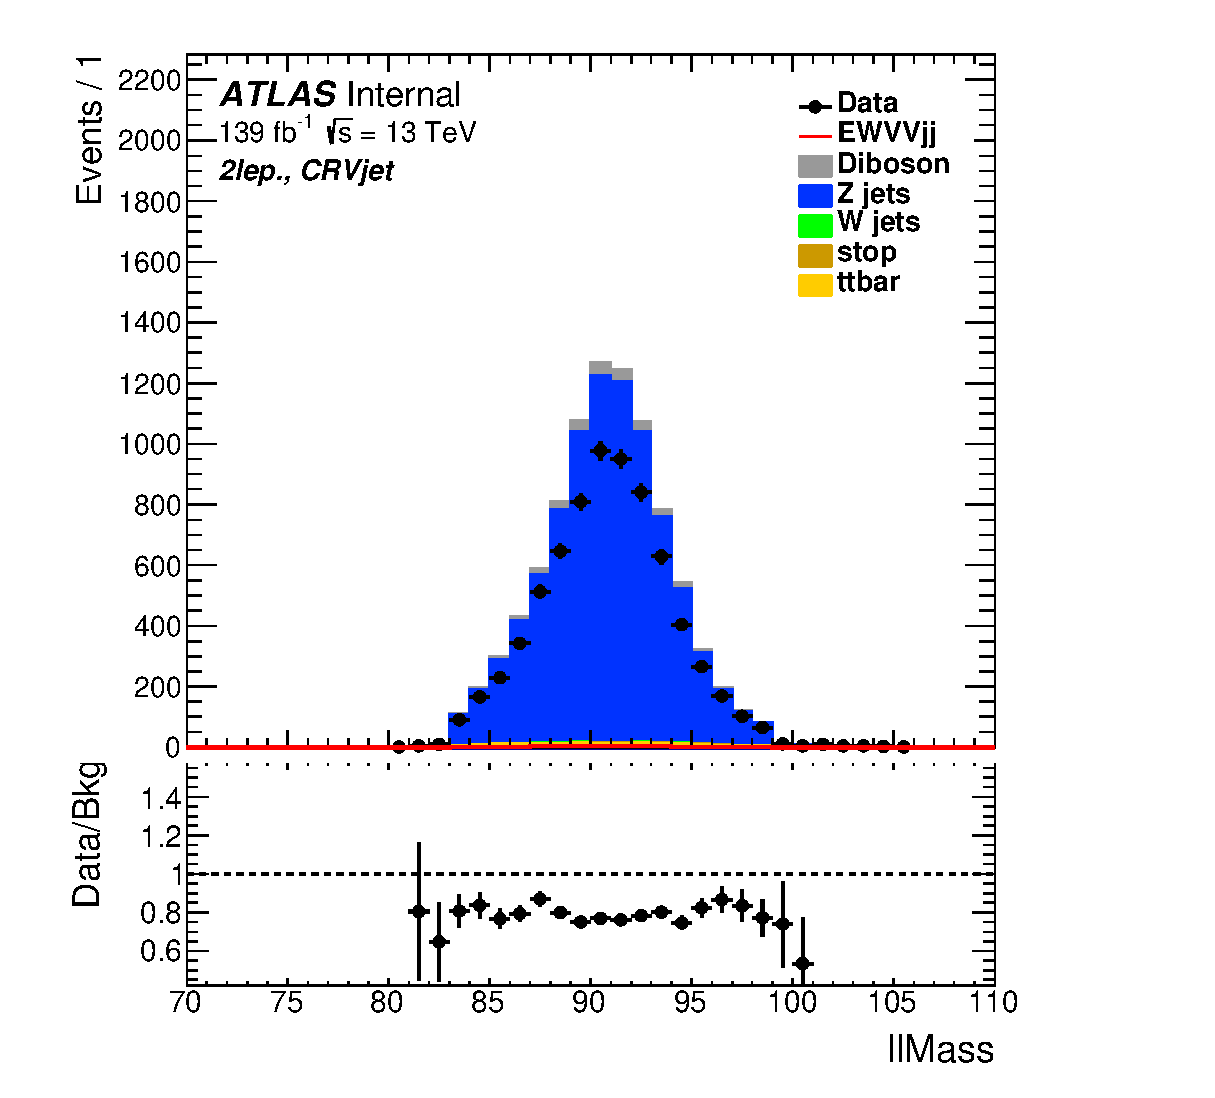
\includegraphics[width=0.30\textwidth]{figures/2lep/reweighting/after_reweighting/C_0ptag1pfat0pjet_0ptv_CRVjet_llMass_Lin.eps}
   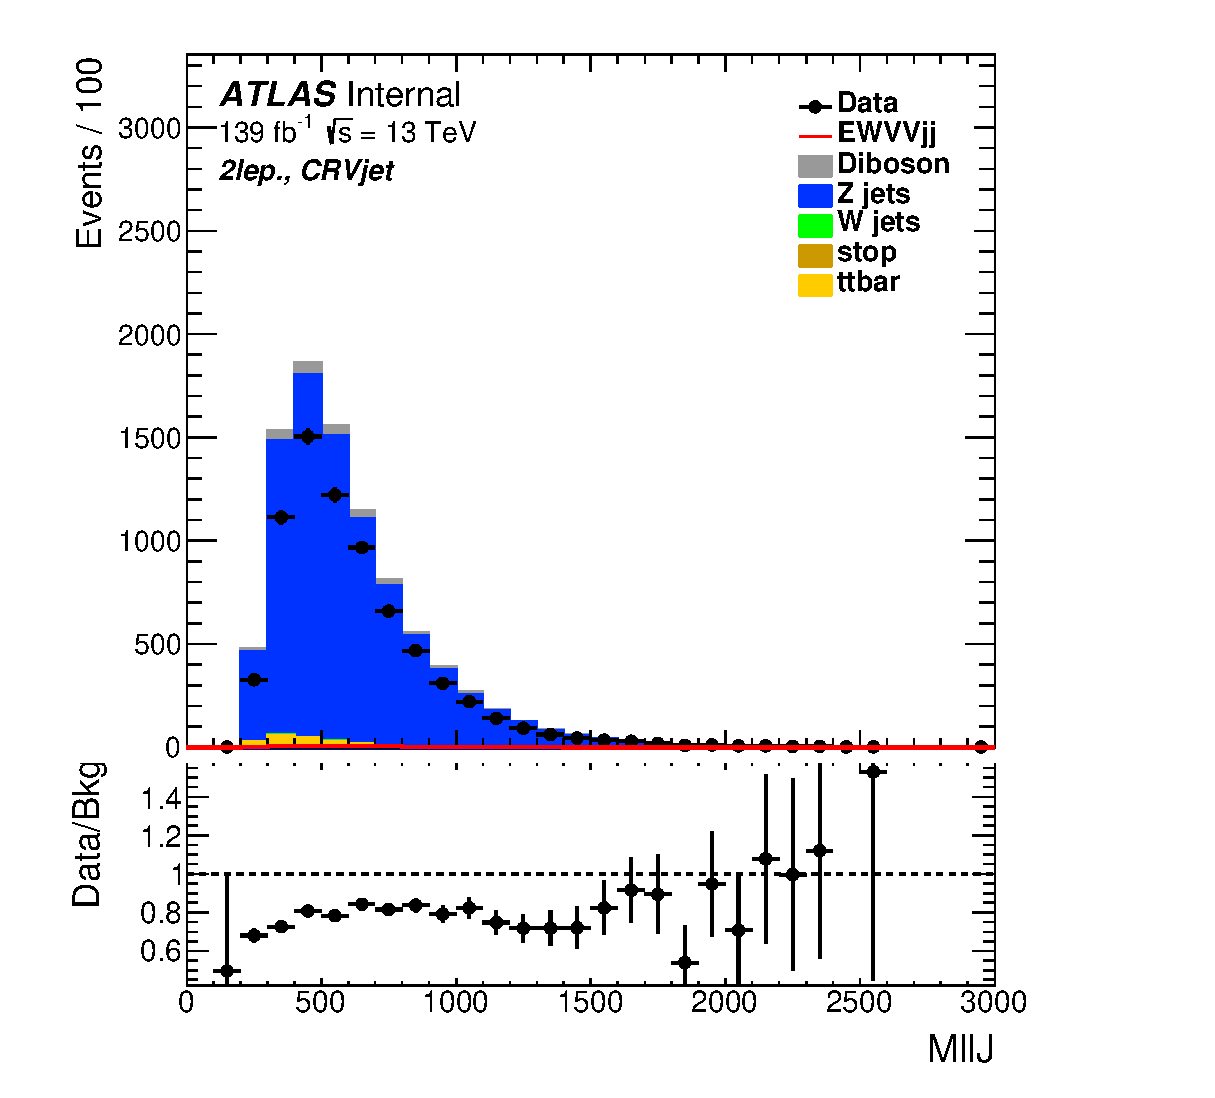
\includegraphics[width=0.30\textwidth]{figures/2lep/reweighting/after_reweighting/C_0ptag1pfat0pjet_0ptv_CRVjet_MllJ_Lin.eps}
   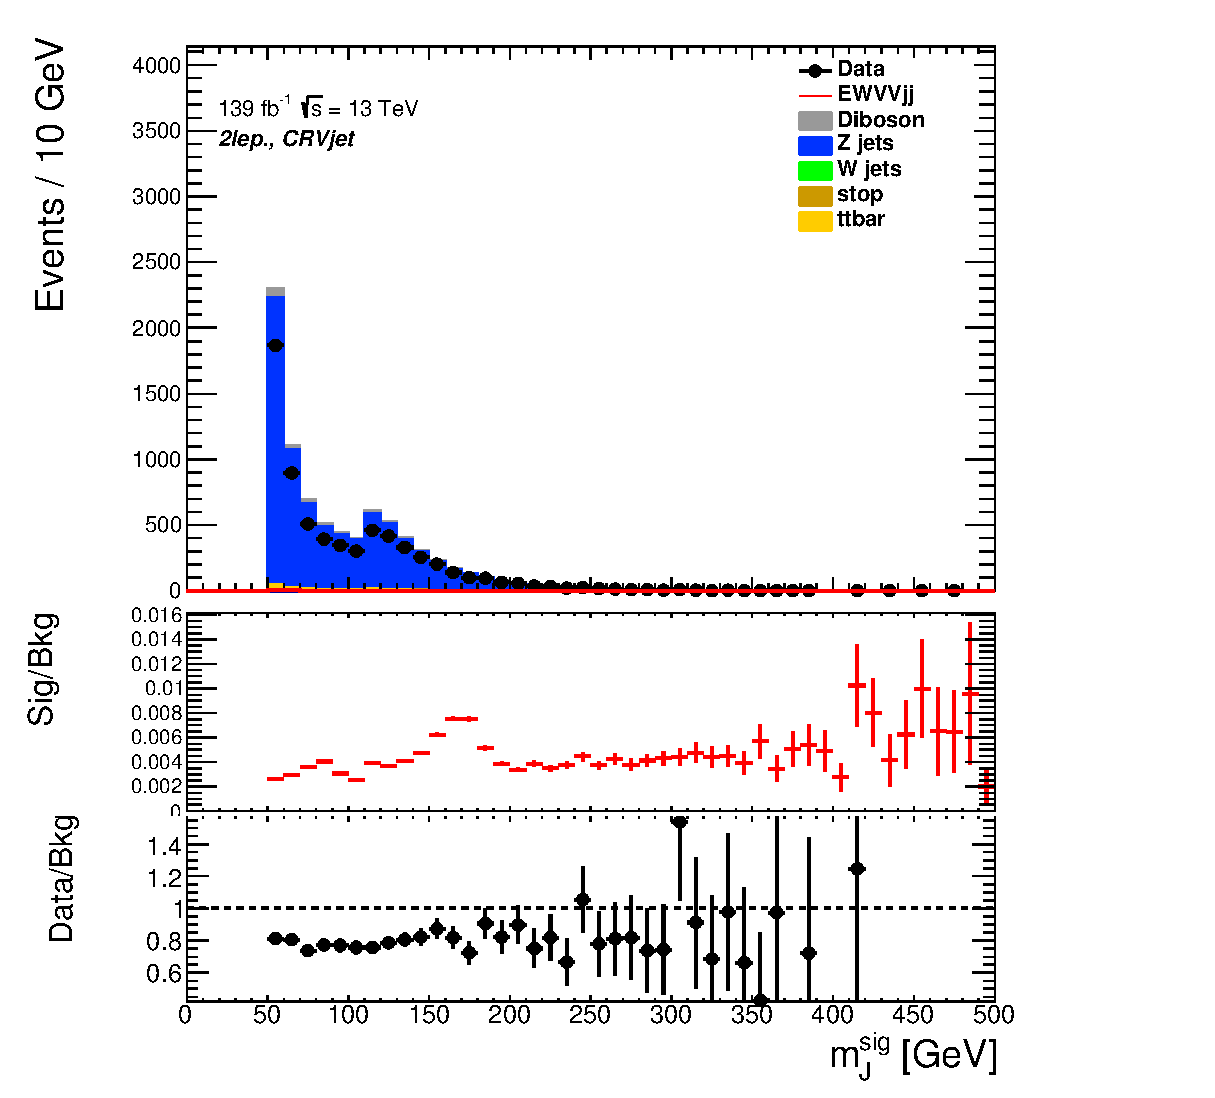
\includegraphics[width=0.30\textwidth]{figures/2lep/reweighting/after_reweighting/C_0ptag1pfat0pjet_0ptv_CRVjet_fatJetMass_Lin.eps}
    \caption{ Various kinematic variables in the Z+jets merged CR in the 2-lepton channel analysis.}
    \label{fig:2lep_zjets_merged_CR}
\end{figure}


% 2-lepton resolved CR fiducial- plots
\begin{figure}[ht]
    \centering
   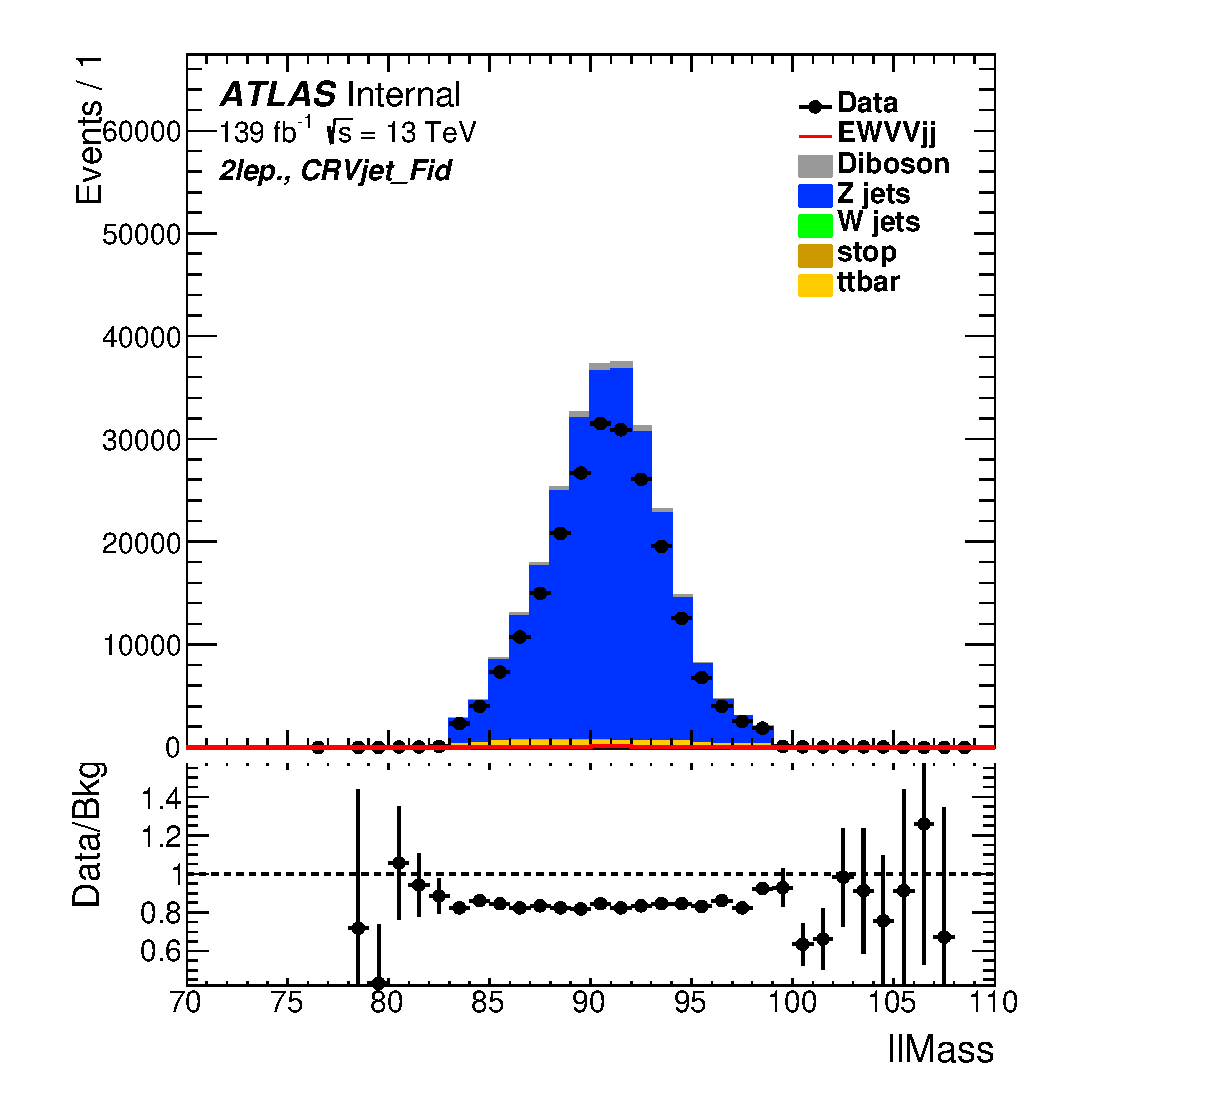
\includegraphics[width=0.30\textwidth]{figures/2lep/reweighting/after_reweighting/C_0ptag2pjet_0ptv_CRVjet_Fid_llMass_Lin.eps}
   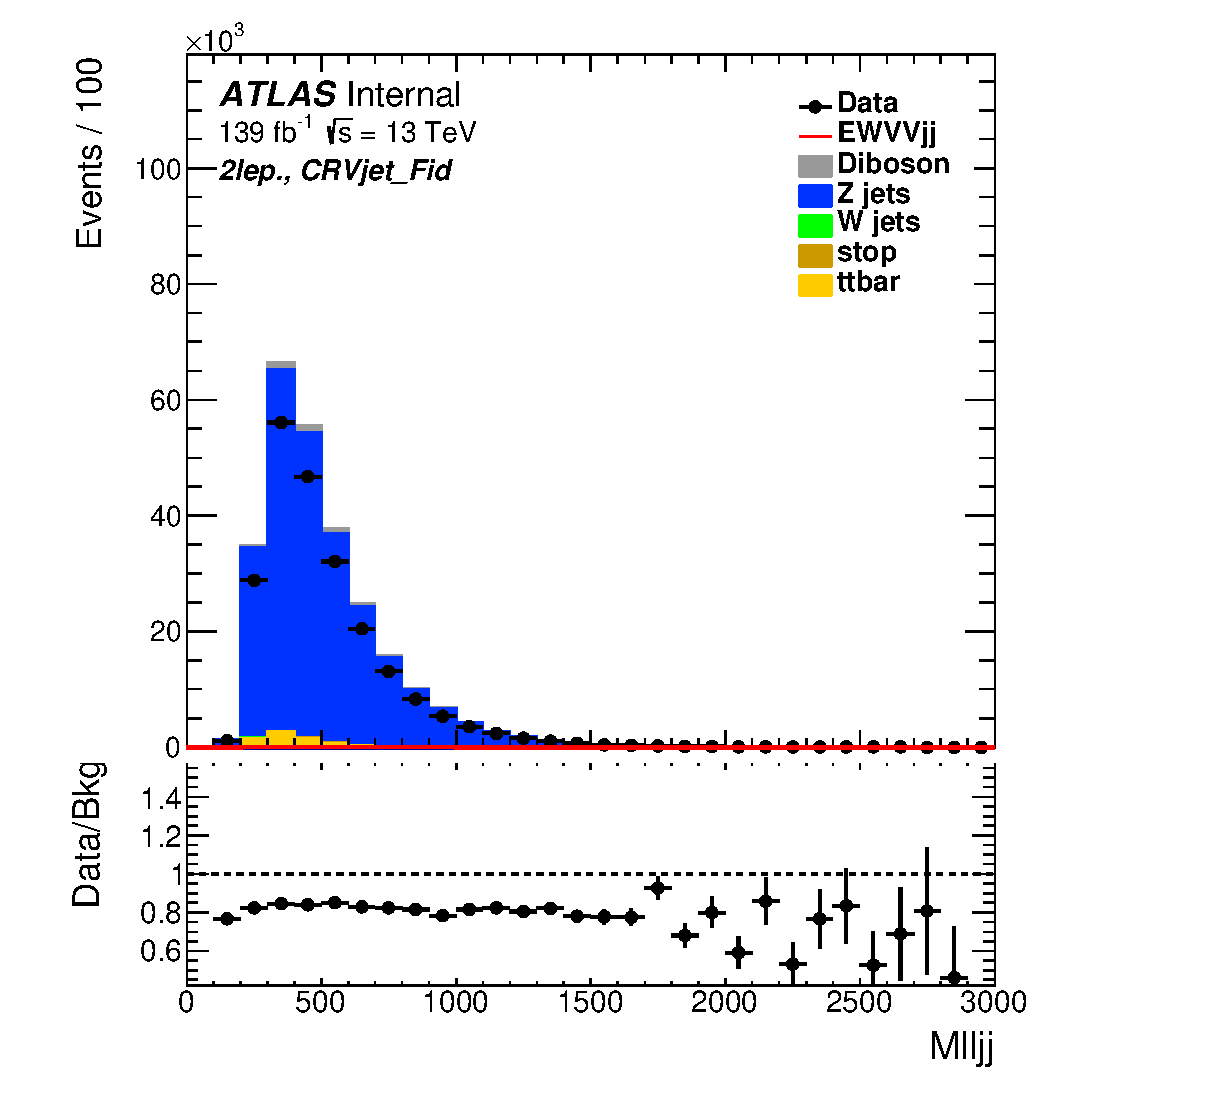
\includegraphics[width=0.30\textwidth]{figures/2lep/reweighting/after_reweighting/C_0ptag2pjet_0ptv_CRVjet_Fid_Mlljj_Lin.eps}
  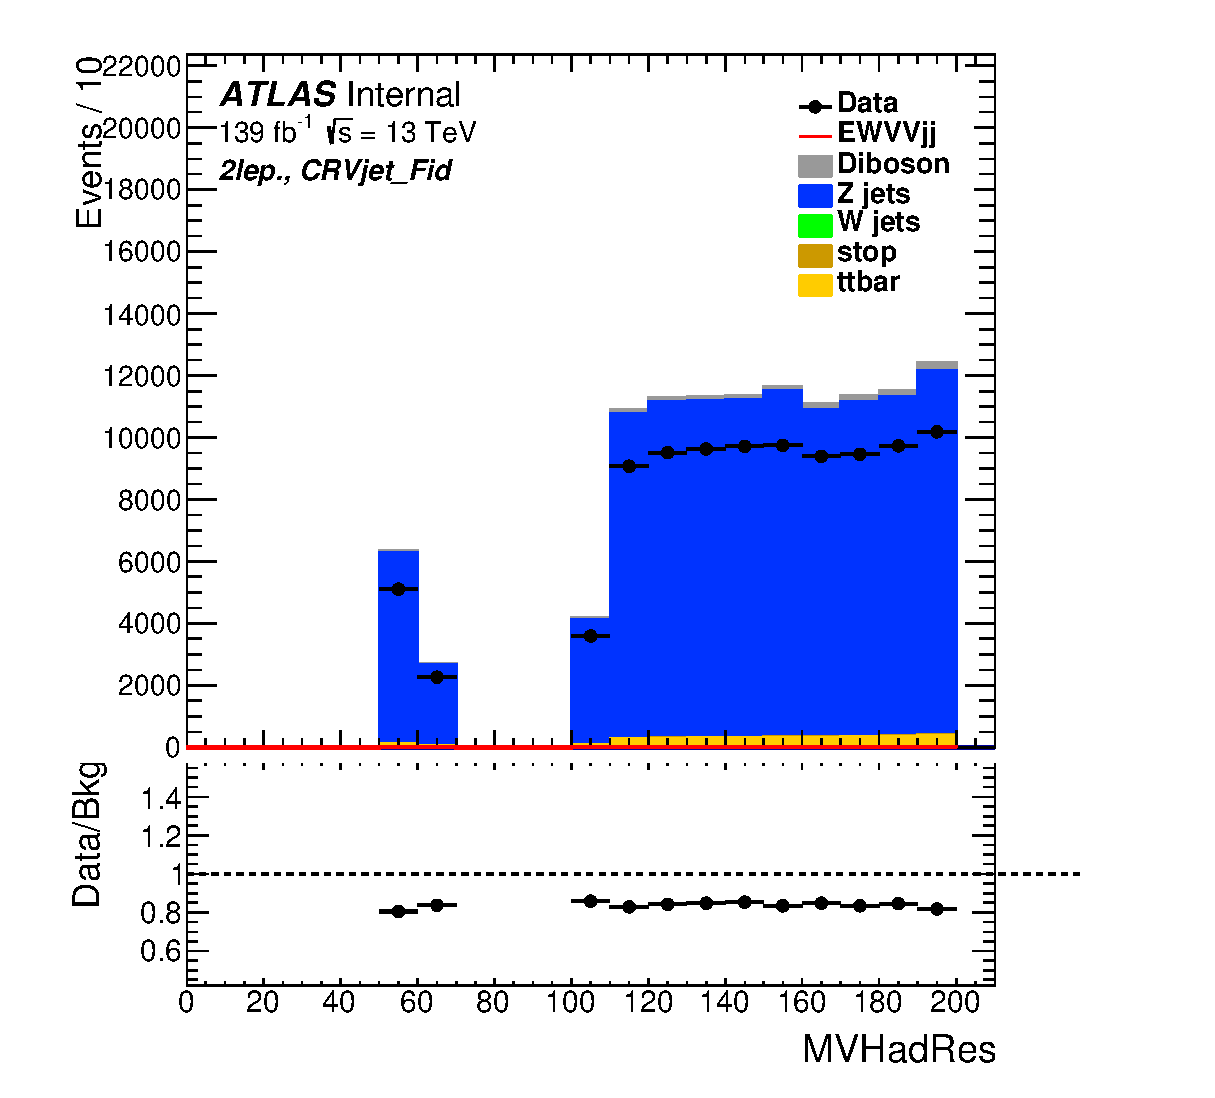
\includegraphics[width=0.30\textwidth]{figures/2lep/reweighting/after_reweighting/C_0ptag2pjet_0ptv_CRVjet_Fid_MVHadRes_Lin.eps}
  \caption{ Various kinematic variables in the Z+jets resolved CR in the 2-lepton channel analysis.}
   \label{fig:2lep_zjets_resolved_CR}
\end{figure}

\section{ttbar modeling}
In 1-lepton channel the ttbar is the dominat background.

